\section{Reporte de funcionalidades}

En esta sección listaremos todas las coberturas que contiene el sistema, contemplando también las que no están documentadas en el informe entregado.

\subsection{Funcionalidades especificadas}
\begin{itemize}
    \item \textbf{RF1 - Gestionar la información básica.} \\
    \textit{Permite la gestión apropiada de la información de la mascota, como es:
    su nombre, peso, altura, posibles comentarios y la imagen.}
    \item \textbf{RF2 - Registrar en calendarios los paseos.} \\
    \textit{Calendario que permite registrar el día y hora de un paseo para una mascota, ingresando el responsable de dicha tarea.}
    \item \textbf{RF3 - Calendario de alimentación de la mascota.} \\
    \textit{Brinda la posibilidad de registrar en el calendario el responsable de alimentar una mascota para un día y hora en especifico.}
    \item \textbf{RF4 - Registro de actividad realizada.} \\
    \textit{Permite registrar una activad ya realizada, la misma puede ser un paseo, alimentación u otra, indicando un nombre, usuario, perro y recorrido o alimento según su tipo.}
    \item \textbf{RF5 - Agendar servicio veterinaria.} \\
    \textit{Funcionalidad que habilita el registar un servicio de cuidado en una veterinaria, como puede ser corte de pelos, uñas, etc.}
    \item \textbf{RF6 - Recordatorios vía email.} \\
    \textit{Envía recordatorio vía correo electrónico y notificaciones de sistema a los responsables de las actividades agendadas previamente.}
\end{itemize}

\subsection{Funcionalidades no especificadas}
\begin{itemize}
    \item \textbf{RF6 - Recordatorios vía email.} \\
    \textit{Carga una colección de datos al sistema para poder operar o probar el resto de su funcionamiento.}
    \item \textbf{RF8 - Agregar usuario.} \\
    \textit{Permite registrar un usuario ingresando nombre y mail, dichos usuarios serán utilizados para la asignación de tareas.}
\end{itemize}


\section{Inventarios de pruebas}

\subsection{Técnicas utilizadas}
Para la siguiente revisión de cobertura de pruebas, se utilizó el componente incorporado en entorno de desarrollo ``IntelliJ IDEA", de esta manera poder obtener la totalidad de lineas de códigos que son comprendidas por las pruebas, mientras que para la verificación de pruebas de caja negra, se tomara como valida únicamente una prueba, siempre y cuando contenga los siguientes elementos:
\begin{itemize}
    \item E1 - Identificador de requerimiento funcional que se prueba
    \item E2 - Requisitos previos.
    \item E3 - Datos de entradas correctos e incorrectos.
    \item E4 - Salida de la prueba esperada.
    \item E5 - Salida de la prueba obtenida.
\end{itemize}

Ponderamos cada uno de estos elementos de igual manera para indicar que una prueba 100\% completa tiene los 5 elementos.

\subsection{Revisión}

\subsubsection{Pruebas de equivalencia}
Para cada una de las funcionalidades nombras en la sección anterior evaluamos la valides de cada una de sus pruebas:

\prettyTable{|p{4cm}|l|l|l|l|l|l|}{
    \textbf{Requerimiento funcional} & \textbf{E1} & \textbf{E2}  & \textbf{E3}  & \textbf{E4}  & \textbf{E5} & \textbf{Cobertura} \\ \hline
    \textbf{RF1} & \xmark & \xmark & \cmark & \cmark & \xmark & 40\% \\ \hline
    \textbf{RF2} & \xmark & \cmark & \cmark & \cmark & \xmark & 60\% \\ \hline
    \textbf{RF3} & \xmark & \cmark & \cmark & \cmark & \xmark & 60\% \\ \hline
    \textbf{RF4} & \xmark & \cmark & \cmark & \cmark & \xmark & 60\% \\ \hline
    \textbf{RF5} & \xmark & \cmark & \cmark & \cmark & \xmark & 60\% \\ \hline
    \textbf{RF6} & \xmark & \xmark & \cmark  & \xmark & \xmark & 60\% \\ \hline
    \textbf{RF7} & \xmark & \xmark & \xmark & \xmark & \xmark & 0\% \\ \hline
    \textbf{RF8} & \xmark & \xmark & \xmark & \xmark & \xmark & 0\% \\ \hline
}


\begin{figure}
    \centering
    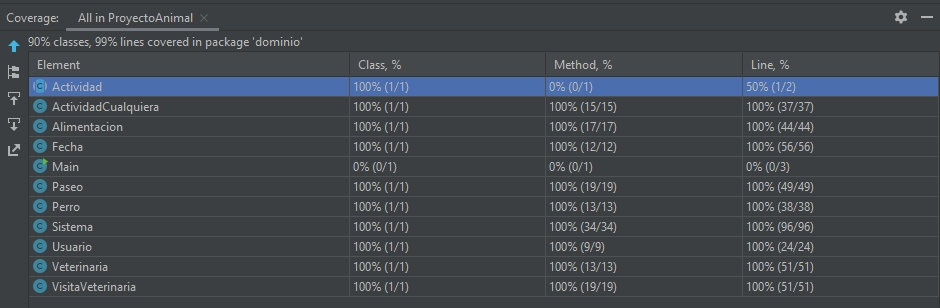
\includegraphics[scale =1.8]{Files/coverturaUnitTests.jpg}
    \caption{Reporte: Cobertura de pruebas unitarias}
    \label{fig:pruebasUnitarias}
\end{figure}
Se observa en la figura: \ref{fig:pruebasUnitarias} que la cobertura de pruebas unitarias es del 90\% de la totalidad del código, siendo que no se puede identificar por este reporte que porcentaje de cobertura tiene cada requisito ficcional, vamos a otorgarle el mismo valor a todos, justificando que las lineas que faltan cubrir pertenecen a métodos que poseen impacto en todos ellos.


\subsubsection{Tabla inventario de pruebas}
\prettyTable{|p{4cm}|p{4cm}|p{4cm}|}{
    \textbf{Requerimiento funcional} & \textbf{Cobertura de las pruebas de caja negra} & \textbf{Cobertura de las pruebas de caja blanca} \\ \hline
    \textbf{RF1} & 90\% &  40\% \\ \hline
    \textbf{RF2} & 90\% & 60\%  \\ \hline
    \textbf{RF3} & 90\% & 60\%  \\ \hline
    \textbf{RF4} & 90\% & 60\%   \\ \hline
    \textbf{RF5} & 90\% & 60\%  \\ \hline
    \textbf{RF6} & 90\% &  60\%  \\ \hline
    \textbf{RF7} & 90\% & 0\%  \\ \hline
    \textbf{RF8} & 90\% & 0\%  \\ \hline
}

\section{Calidad de codificación}

\subsection{Estilo de codificación}
En esta sección se analizara el reporte de la figura \ref{fig:PMD}, el cual permite observar que existen 242 violaciones a las buenas practicas de la programación, 175 al ``codeStyle " y 55 a estándares de diseño, siento la totalidad de lineas de código 2446, se puede afirmar que la calidad generar del código es mala, generando que el actual estado genere mayor dificultad al mantenimiento del sistema, y aumente las horas de desarrollo de nuevas funcionalidades y los costos asociados.



\begin{figure}[H]
    \centering
    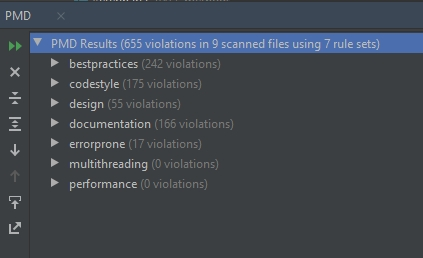
\includegraphics[scale =3]{Files/analisisPMD.jpg}
    \caption{Reporte: PMD}
    \label{fig:PMD}
\end{figure}

\subsection{Complejidad de la aplicación y otros factores}
Además de realizar un análisis de estilo de código se utilizó la herramienta CodeMR, el cual es una herramienta integrada en la suite de programación Intellij Idea, la cual muestra una grán cantidad de métricas para el código, y ciertos resúmenes de complejidad, de los cuales se puede observar que la complejidad de la clase sistema es muy superior a la de las demás clases, esto podria ser algo esperado ya que es la clase central, pero también nos muestra como esta clase es muy grande ya que tiene una grán cantidad de líneas de código(LOC: 126) y una grán cantidad de métodos(WMC: 61), esto representa que roba mucha funcionalidades de las que debería encargarse el dominio.
\begin{figure}[H]
    \centering
    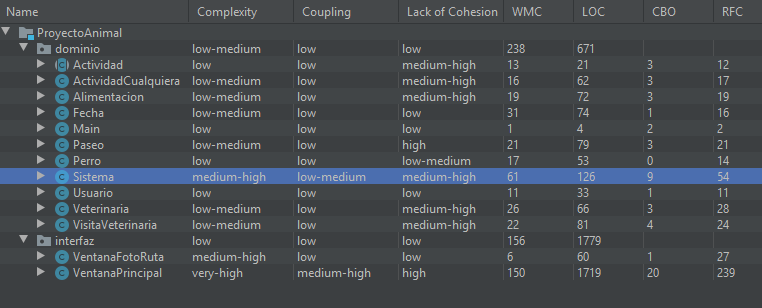
\includegraphics[scale =0.5]{Files/codeMR.png}
    \caption{Reporte: CodeMR}
    \label{fig:MR}
\end{figure}

\section{Resumen}

Luego de finalizados las tareas de análisis, se puede afirmar que la documentación esta incompleta, no reflejando la totalidad de las funcionalidades que el software contiene, sin casos de usos de los mismos y pruebas de equivalencia incompletas en su estructura. De igual modo, el código de fuente de este software, incumple con estándares de codificación como se menciono en la sección anterior, contiene varios errores reportados no corregidos, como también errores no reportados. Además la distribución de la complejidad no es buena al haber clases muy complejas trabajando con clases muy sencillas.\\
Se puede resumir que el estado actual del proyecto es malo, dificultando de esta manera el mantenimiento del mismo, y haciendo compleja la implantación de nuevas funcionalidades.